
\section{Nvidia Pascal architecture \cite{nvidia:pascalwhitepaper}}
In April 2016, the Nvidia Pascal architecture was presented.
Nvidia's most powerful chip using this architecture is called GP100, which they have built into the Tesla P100 Accelerator.

The Tesla P100 has 5.3TFLOPS of FP64 performance, double as much (10.6 TFLOPS) of FP32, and up to four times as much (21.2 TFLOPS) of FP16.
The 16-bit floating point precision ability is thought for Deep Learning, which was the focus at Nvidia's presentation, althought it could also be useful for graphics.
Deep Learning does not require higher precision and this brings both higher speed and higher available storage for bigger models.

In the following sections the main features of the new architecture are described.
All of them are present in the Tesla P100 Accelerator.

% \subsection{Microprocessor architecture}
\subsection{Updated processor structure}
\begin{figure}[ht!]
    \centering
    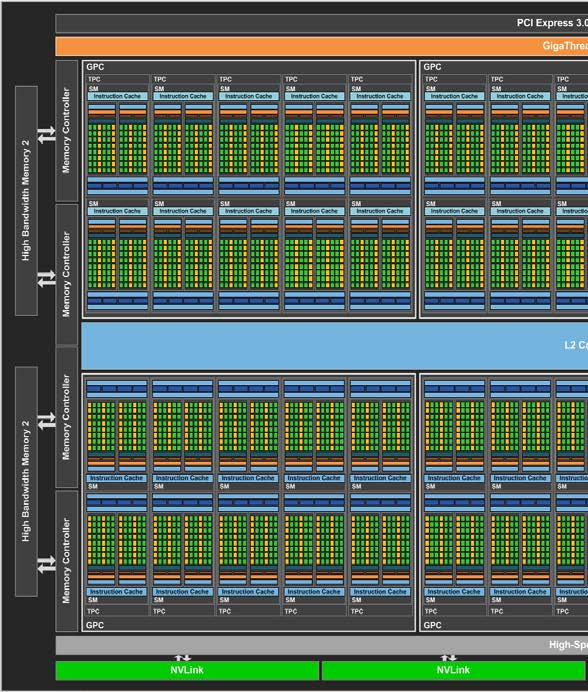
\includegraphics[width=\linewidth]{gp100_half}
    \caption{Representation of half of the GP100 Pascal silicon chip. The right half is
             completely symmetric. \cite{nvidia:pascalwhitepaper}}
    \label{fig:gp100}
\end{figure}

The Pascal architecture is structured as an array of Graphics Processing Clusters, each GPC is formed by several Texture Processing Clusters, consisting of 2 Streaming Multiprocessors per TPC.
The reason for conceptually grouping 2 Streaming Multiprocessors into one Texture Processing Cluster is not specified.
The GP100 processor has 6 Graphics Processing Clusters with 10 Streaming Multiprocessors each.
Each Streaming Multiprocessor contains 64 CUDA FP32 Cores and 4 texture units (see Figure \ref{fig:sm}).
This adds up to a total of 3840 CUDA Cores (6 $\times$ 10 $\times$ 64)
However, 4 of the Streaming Multiprocessors on the chip are turned off, giving a total of 56 available Streaming Multiprocessor units.

\begin{figure}[ht!]
    \centering
    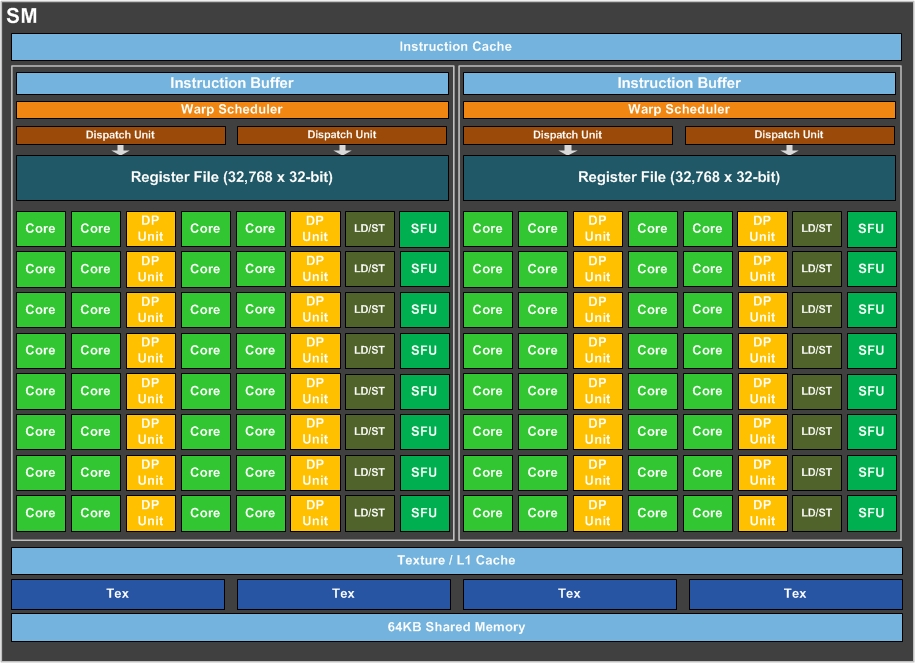
\includegraphics[width=\linewidth]{gp100_sm}
    \caption{Representation of a Pascal Streaming Multiprocessor capable of simultaneously executing two sets of 32 threads}
    \label{fig:sm}
\end{figure}

Each Streaming Multiprocessor has two sets of 32 FP32 CUDA Cores, an instruction buffer, and a warp scheduler with two dispatch units.

There is a new scheduler data path too.
As in older architectures, each warp scheduler in Pascal Streaming Multiprocessors can dispatch two independent instructions simultaneously.
There is also a 1:2 ratio of FP64 to FP32 CUDA Cores per Streaming Multiprocessor, working better with the updated data path.
FP16 is handled by the same FP32 ALUs.

The minimum block size for FP32 remains of 32 threads.
The minimum block size for FP16 and FP64 is not specified.

\subsection{Compute Preemption}
The GP100 chip has preemption at instruction-level.
It allows interaction with long computing tasks, swapping contexts to GPU DRAM.
Otherwise, long running tasks could end up being killed by the OS or the CUDA driver.
Additionally, if a GPU is being used for display graphics and CUDA tasks, long running tasks could result in an unresponsive GUI.
This does not happen anymore.
This also makes interactive debugging work better.
Interactive debugging on Kepler and Maxwell required adding instrumentation during compilation to allow completion of thread blocks after an interrupt.
Thus GP100 debugging is more robust and lightweight.

\subsection{Memory}
\subsubsection{On-chip memory}
As in previous architectures, memory is structured hierarchically.
There are two cache levels --- L1/shared and L2 --- which improve access to off-chip memory.

The L1/shared memory structure has not changed since Maxwell.
Each Streaming Multiprocessor disposes of 64KB shared memory --- up to 32KB per Thread Block.
L1/texture cache is additional to that.
The Register File Size per Streaming Multiprocessor remains at 256KB.
It should be noted that the number of cores per Streaming Multiprocessor has been at least halved compared to previous architectures, while the number of Streaming Multiprocessors increases.
A summary of this evolution can be seen in Figure \ref{fig:cuda_cores}.
All this additional fast memory improves thread concurrency capabilities.

There are eight 512-bit memory controllers to communicate with off-chip memory, as seen on the left side of Figure \ref{fig:gp100}.
There is a unified 4096KB L2 cache, which gives 512KB per memory controller.

\subsubsection{Off-chip memory --- HBM2}

\begin{figure}[ht!]
    \centering
    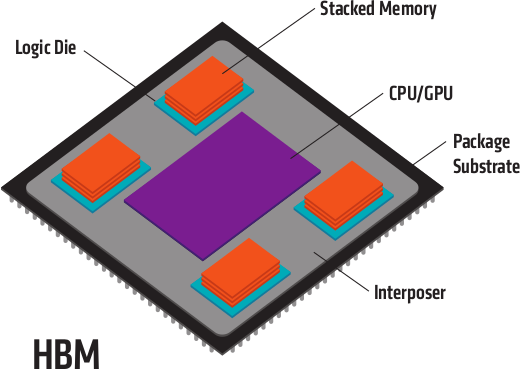
\includegraphics[width=\linewidth]{hbm}
    \caption{Chip structure using HBM memory \cite{amd:hbm}. The memory and the chip share a silicon interposer connection \cite{amkor:hbmwhitepaper}.}
    \label{fig:hbm}
\end{figure}
HBM2 is the second generation of High Bandwidth Memory.
HBM is the first 3D-memory technology to be in broad use.
Each stack of HBM2 is controlled by a pair of memory controllers.
A HBM2 stack can be composed by 4 or 8 dies with perpendicular microscopic wires (called through-silicon vias) that go down the stack.
Each HBM2 die has a 8Gb capacity, giving a total of 4 or 8GB per stack.
This distribution enables a higher number of connections, increasing the communication bandwidth.
Stacked memory uses less surface, which also allows for denser servers.
The Tesla P100 uses 4 stacks of 4 dies, providing with 16GB of memory.

Each die is connected through two 128-bit channels.
These channels are independent and not necessarily asynchronous.
The stacks are connected to the chip via a passive silicon interposer (see Figure \ref{fig:hbm}).
It is a large piece of passive silicon also using through-silicon vias (TSVs) for connections.
This means a large silicon surface, which is expensive.
That is why lower-range Pascal cards --- such as graphics oriented GTX1080 --- will use GDDR5 or GDDR5X.
The height of the dies is adjusted --- the top die is thicker --- in order to make good contact with the heat sink.

HBM2 is a significant scale up on its previous version.
HBM1 supported only 4 dies per stack and 2Gb per die.
HBM1 supported 125GB/sec per stack while HBM2 supports 180GB/sec.

When working on large clusters or having long application executions, it becomes important to have a memory error correction system.
HBM2 has native support for ECC.
This contrasts with GDDR5 which does not have internal ECC, which only allows ECC to detect error on the bus.
This approach requires allocating an 6.25\% of the memory for error correction, and results in a 12-15\% reduction in bandwidth.
Internal ECC detects and corrects single-bit soft errors before they affect the system, without requiring to reserve some of the memory for this function.

Another relevant incorporation is a new block on the chip called High-Speed Hub (HSHUB) --- on the bottom of Figure \ref{fig:gp100} --- which has access to the High-Speed Copy Engines enabling NVLink access.
NVLink is an important addition that makes working with Unified Memory more efficient.

\subsubsection{Unified Memory}
The path to Unified Memory is being followed since several CUDA versions ago.
CUDA 4 introduced Unified Virtual Addressing.
Unified Virtual Addressing enabled pinning CPU memory to be accessible directly over PCIe without a memcpy.
This provided convenience but no performance improvement.

The term Unified Memory was introduced in CUDA 6.
In CUDA 6, not only is pinned memory accessible through PCIe, but a single pointer can refer to both CPU and GPU memory.
This requires pinned CPU memory to be associated with GPU memory of the same size, and limits the unified address space to the size of GPU memory.
A single memory allocation in pinned CPU memory and GPU memory is kept synchronized through software.
As described in section \ref{subsec:unifmemanaly}, all managed memory touched by the CPU has to be synchronized.
Additionally, CPU and GPU cannot access the same memory allocation simultaneously.

Together with Pascal and NVLink, the CUDA 8 platform has been released.
Now a single memory address space for CPU and GPU with 49-bit virtual addressing has been introduced.
Since current CPUs have up to 48-bit virtual addressing, 49 bits is enough to cover both spaces as a single virtual address space.
Now the memory limits of the GPU do not restrict the virtual space size.
Additionally, the GP100 chip has hardware support for page faulting, which allows transparent access to data anywhere in the virtual address spaces.
This means there is no need for synchronization of all managed memory allocations.
The large address space allows direct addressing of very large datasets, much larger than the system memory.
Faulted pages are automatically migrated.
Pages can also be mapped on the GPU for access through PCIe or NVLink.
In some cases, this can be faster than migrating.
CPUs can also fault and migrate memory from GPU.
CPU can even access data while a GPU kernel is running.
Coherency in this case could not be guaranteed in previous architectures.
Note that correct synchronization has to be taken care of as in any other parallel application.

Operating system support is being developed in collaboration with Red Hat and the Linux community to enable GPUs to access memory allocated with the default OS allocator, such as malloc.

Aside from making GPU programming easier, this also allows easier use of C++ classes on GPU.
Any nested data can be automatically accessed thanks to the single virtual address.

It is important to note that Unified Memory can easily lead to communication bottlenecks.
In order to alleviate this problem, Nvidia has developed NVLink.

\subsection{NVLink}

Clusters of multi-GPU systems are being interconnected with InfiniBand(R) and 100Gb Ethernet.
The GPUs to CPUs ratio is increasing.
Fast cluster interconnections and this increasing ratio are causing PCIe to become a significant bottleneck for data-intensive tasks.
That is why NVLink has been developed.

\subsubsection{Previously existing features}
RDMA has already been possible for some time.
GPUDirect was introduced in Kepler and allowed RDMA, lowering CPU overhead.
This is thanks to the CPU not having to copy the data inside its own memory.
It also enabled P2P data transfer between GPUs.
GPUDirect bandwidth is doubled in GP100.
\subsubsection{NVLink features}
NVLink introduces GPU-to-GPU data transfers, avoiding both CPU overhead and PCIe bottlenecks at once.
It uses the new Nvidia High-Speed Signaling (NVHS) interconnect.
It is compatible with the GPU ISA, supporting shared memory multiprocessing.
Programs can execute directly on memory of another GPU with full capabilities.

Additionally, CPU-to-GPU NVLink connections will also be possible for compatible CPUs.
The connection to non-supporting CPUs will still happen through PCIe.
The ``Power8 with NVLink'' processor is the first processor supporting the technology.
It was previously known as Power8+.
``Power8 with NVLink'' has 6 NVLink connectors, allowing for multiple network topologies \cite{openpower:roadmap}.
The next generation Power9 will support both NVLink and IBM's own CAPI \cite{openpower:interconnect2016}.
It will be launched in 2017.
An schematic of this processor series can be seen in Figure \ref{fig:nvlpower}.

\begin{figure}[ht!]
    \centering
    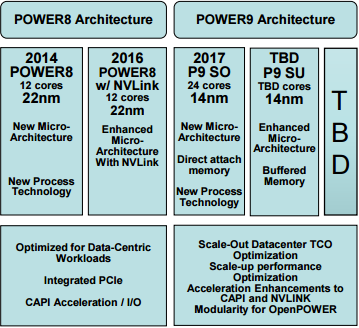
\includegraphics[width=\linewidth]{NVLink_Power}
    \caption{IBM NVLink supporting processors timeline [OpenPower Foundation]}
    \label{fig:nvlpower}
\end{figure}

This processor together with Nvidia GPUs will be the building blocks of the pre-exascale Summit and Sierra supercomputers.
This is described in section \ref{subsec:nvlsupercomp}.
These supercomputers will be the first using Volta, Nvidia's next generation GPU architecture.
This will be in 2017.
However a broader launch of Volta GPUs is not expected until 2018.
No Intel processor support for NVLink is expected as of June 2016.
This is probably due to Intel's Xeon Phi processor series, a competitor to GPU accelerators.
Xeon Phi follows a different approach for hardware accelerators.

\subsubsection{NVLink design}
Data is transmitted over a set of differential pairs with a bandwidth of 20Gb/sec each pair.
A total of 16 pairs form a Link, with 8 pairs for each direction.
This results in a total bidirectional bandwidth of up to 40GB/sec per Link.
It is important to remark that this is bidirectional because there has been some confusion with this.
PCIe Gen 3 x16 --- the current technology in use --- provides a bidirectional bandwidth of up to 31.75GB/s.
In this way NVLink is just about 20\% faster than PCIe, and slower than PCIe 4.0 which doubles the bandwidth of PCIe 3.0.
However it is NVLink's capability of joining several links to add up their bandwidths what makes it really faster.
Since the Tesla P100 supports up to 4 links, this allows up to 160GB/sec bidirectional data transfer.
A couple of Tesla P100 cards can thus be connected with a bandwidth of up to more than 5x that of PCIe 3 x16.
While a single link of NVLink has smaller bandwidth than PCIe 4.0, a NVLink 2.0 specification is expected for 2017, improving on PCIe 4.0 \cite{nextplatform:nvlink}.
NVLink also uses up to a third of the energy to move data compared with PCIe Gen3 x16 \cite{nvidia:hpcnvlink}.

\subsubsection{NVLink layer model}
The NVLink controller is formed by a Physical Layer, a Data Link Layer, and a Transaction Layer.
The package sizes range from 1 to 18 128-bit flits.
The clock runs at 1.25GHz.
It uses an embedded clock used by the receiver to capture data.
The Physical Layer takes care of deskewing across lanes, framing, scrambling/descrambling, polarity inversion and lane reversal.
The Data Link Layer is responsible for reliable transmission.
Packets are protected with a 25-bit Cyclic Redundancy Check.
It is calculated over the current header and the previous payload.
It allows detection of up to 5 random bit errors or up to 25-bit bursts of errors on any lane.
Packets are stored in a replay buffer until the receiver acknowledges them.
If the transmitter times out waiting for acknowledgment, it starts retransmitting.

The Transaction Layer cares for synchronization, link flow control, and virtual channels.
It can also aggregate multiple links together to provide higher communication bandwidth.

\section{NVLink performance}
In \cite{nvidia:nvlinkperformance}, a basic performance analysis on NVLink is presented.
Since it was done in 2014, the analysis was done on a theoretical basis.
It focuses on the performance benefits for GPU-to-GPU communications through NVLink.
Two systems with and without NVLink are analyzed for the different cases.
The systems with NVLink can be seen in Figure \ref{fig:nvlinkconfigs}.
The base case systems are the same just removing the NVLink connections.
It assumes a 80\% communication efficiency for both PCIe and NVLink.

\begin{figure}[ht!]
    \centering
    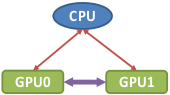
\includegraphics[width=0.45\linewidth]{2gpus}\\
    \vspace*{0.5cm}
    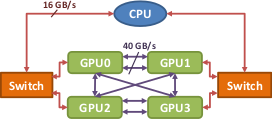
\includegraphics[width=0.8\linewidth]{4gpus}
    \caption{Two possible NVLink + PCIe configurations}
    \label{fig:nvlinkconfigs}
\end{figure}

The theoretical test-cases are a multi-GPU exchange and sort, a Fast Fourier Transform, AMBER-Molecular Dynamics, ANSYS Fluent, and a Lattice Quantum Chromodynamics library.
The exchange and sort case achieves an improvement directly proportional to the parallel communication speed-up.
The FFT case shows that NVLink also makes multi-GPU scaling worth for smaller problems by reducing the communication/computation time ratio.
AMBER's PMEMD algorithm can be decomposed into a N-body simulation and a FFT which can run asynchronously.
This is already a complex case to analyze, but it is estimated that a 30-50\% improvement for 4 GPUs can be achieved just by using NVLink.
In the ANSYS Fluent case an improvement of 25\% for 2 GPUs is expected to be achieved through a synchronous communication speed-up.
In the LQCD case, the speed-up depends on the memory bandwidth, the interconnect bandwidth and the surface-to-volume ratio of the computation.
It is estimated that a 25\% improvement for 4 GPUs is also to be expected.
